%----------------------------------------------------------------------------------------
%	RESULTS
%----------------------------------------------------------------------------------------

\begin{exampleblock}{Results}

\begin{figure}
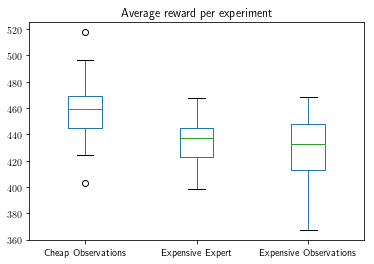
\includegraphics[width=0.45\linewidth]{img/avg_reward.png}
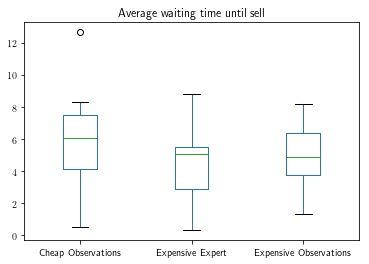
\includegraphics[width=0.45\linewidth]{img/avg_waiting.png}
\caption{Average reward and waiting times in different experiment scenarios.}
\end{figure}

\begin{figure}
    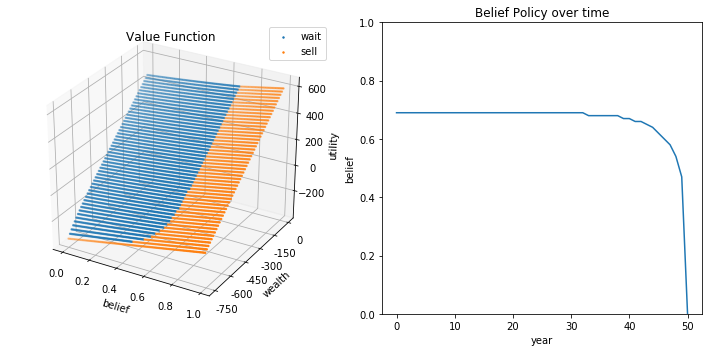
\includegraphics[width=0.8\linewidth]{img/rational_policy.png}
\caption{Value function and policy of a traditional RL agent with risk-neutral behaviour in the expensive observation scenario. The agent sells at a fixed belief regardless of waiting time.}
\end{figure}

\begin{figure}
    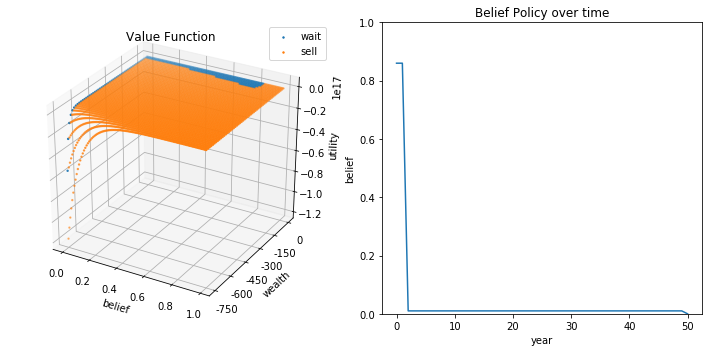
\includegraphics[width=0.8\linewidth]{img/sine_policy.png}
    \caption{Value function and policy of a RL agent with hyperbolic sine utility function in the expensive observation scenario. The agent sells at a fixed time step regardless of its belief.}
\end{figure}

\begin{figure}
    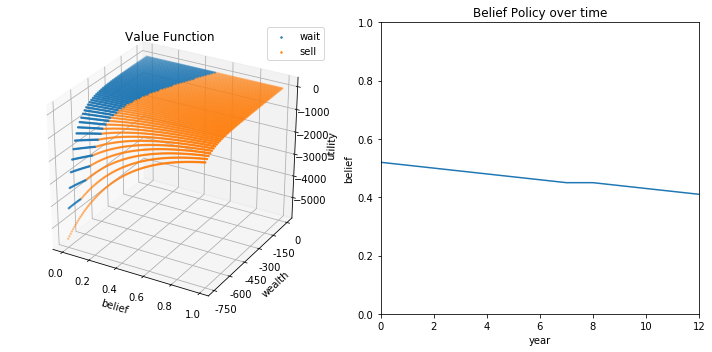
\includegraphics[width=0.8\linewidth]{img/dynamic_policy.png}
    \caption{Value function and policy of a RL agent with hyperbolic sine utility function in the expensive observation scenario. The agent sells depending on both time and its belief.}
\end{figure}


\begin{figure}
    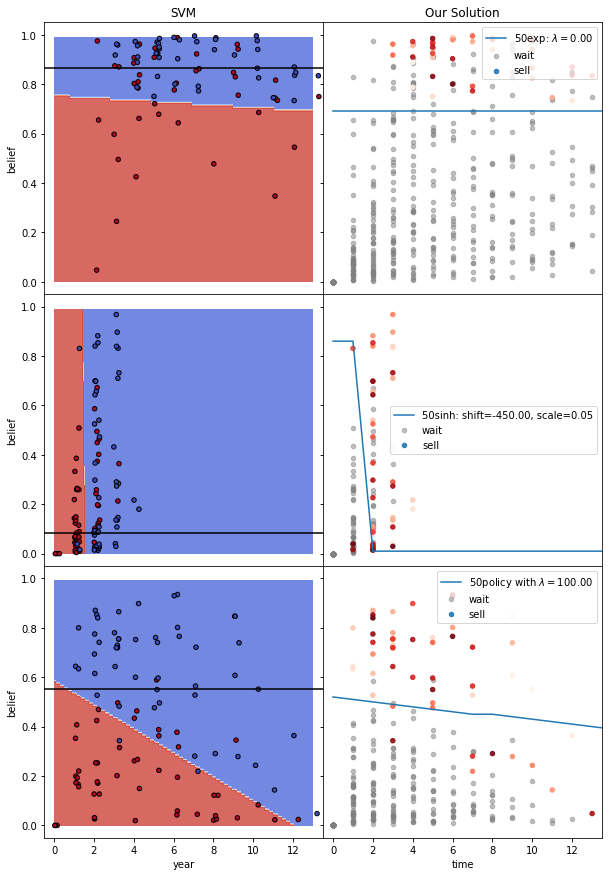
\includegraphics[width=0.8\linewidth]{img/fit.png}
\caption{Examples from three different behaviors observed and replicated with RL agents.}
\end{figure}
